%1テストデータについて
\begin{deletedblock}
Test data were acquired for the four types of postures: mouse operation, pad operation, sitting still, and typing, as for training data. 
As for mouse operation, the posture of the subjects was captured for 30 seconds as they manipulated a mouse to write the alphabet in order from ``A'' to ``Z''. The capturing was performed only once to acquire test data.
As for pad operation, the posture of the subjects was captured for 30 seconds as they performed a pad operation on the PC to write the alphabet in order from ``A'' to ``Z''. The capturing was performed only once to acquire test data. 
As for sitting still, the posture of the subjects was captured for ten seconds as they sat still without moving and did not touch the PC. The capturing was performed only once to acquire test data. 
As for typing, the posture of the subjects was captured for 30 seconds as they typed the alphabet in order from ``A'' to ``Z''. The capturing was performed only once to acquire test data.
\end{deletedblock}

\deleted{Test data were acquired for the four posture classes under the conditions summarized in Table~\ref{dataacquisition}; each capture was performed once per subject.}
\revised{Test data were acquired for the four posture classes under the conditions summarized in Table~\ref{dataacquisition}; each capture was performed once per experiment participant.}
\deleted{Test data were acquired for the four posture classes under the conditions summarized in Table~\ref{testacquisition}; each capture was performed once per subject.}
\begin{deletedblock}
\begin{table}[b]
  \centering
  \caption{Test data acquisition conditions for each posture class.}
  \label{testacquisition}
  \scalebox{0.9}{
  \begin{tabular}{l|l|c}
    \hline
    Posture class & Task & Duration \\ \hline
    Mouse operation & Write alphabet A--Z using mouse & 30 s \\
    Pad operation & Write alphabet A--Z using trackpad & 30 s \\
    Sitting still & Sit still without moving or touching PC & 10 s \\
    Typing & Type alphabet A--Z on keyboard & 30 s \\
    \hline
  \end{tabular}
  }
\end{table}
\end{deletedblock}

%6テストデータの被験者
\revised{We used 28 experiment participants from the 31 experiment participants.}
  \revised{The 28 experiment participants were not sampled for training.}
\deleted{The 28 subjects in this study are denoted as subjects A to AB.}
\revised{The 28 experiment participants in this study are denoted as experiment participants A to AB.}
    %6-1テストデータの名称（データセット別名は削除）
    \deleted{Test data with subjects A to AB is called test data A to AB.}
    \deleted{Test data with experiment participants A to AB is called test data A to AB.}

% \end{spverbatim}
 
% \begin{figure}[ht]
%   \centering
%   \subfloat[Left LiDAR sensor]{
%     \includegraphics[width=.6\linewidth]{img/pcleft.png}
%     \label{pcleft}
%   }
%   \\
%   \subfloat[Right LiDAR sensor]{
%     \includegraphics[width=.6\linewidth]{img/pcright.png}
%     \label{pcright}
%   }
%   \\
%   \subfloat[Both LiDAR sensors]{
%     \includegraphics[width=.6\linewidth]{img/pcmerge.png}
%     \label{pcmerged}
%   }
%   \caption{Visualization of data from each LiDAR.}
%   \label{eachlidar}
% \end{figure} 
 
%6/27 tb ⇒ t
\begin{figure}[t]
  \centering
  \subfloat[Mouse operation]{
    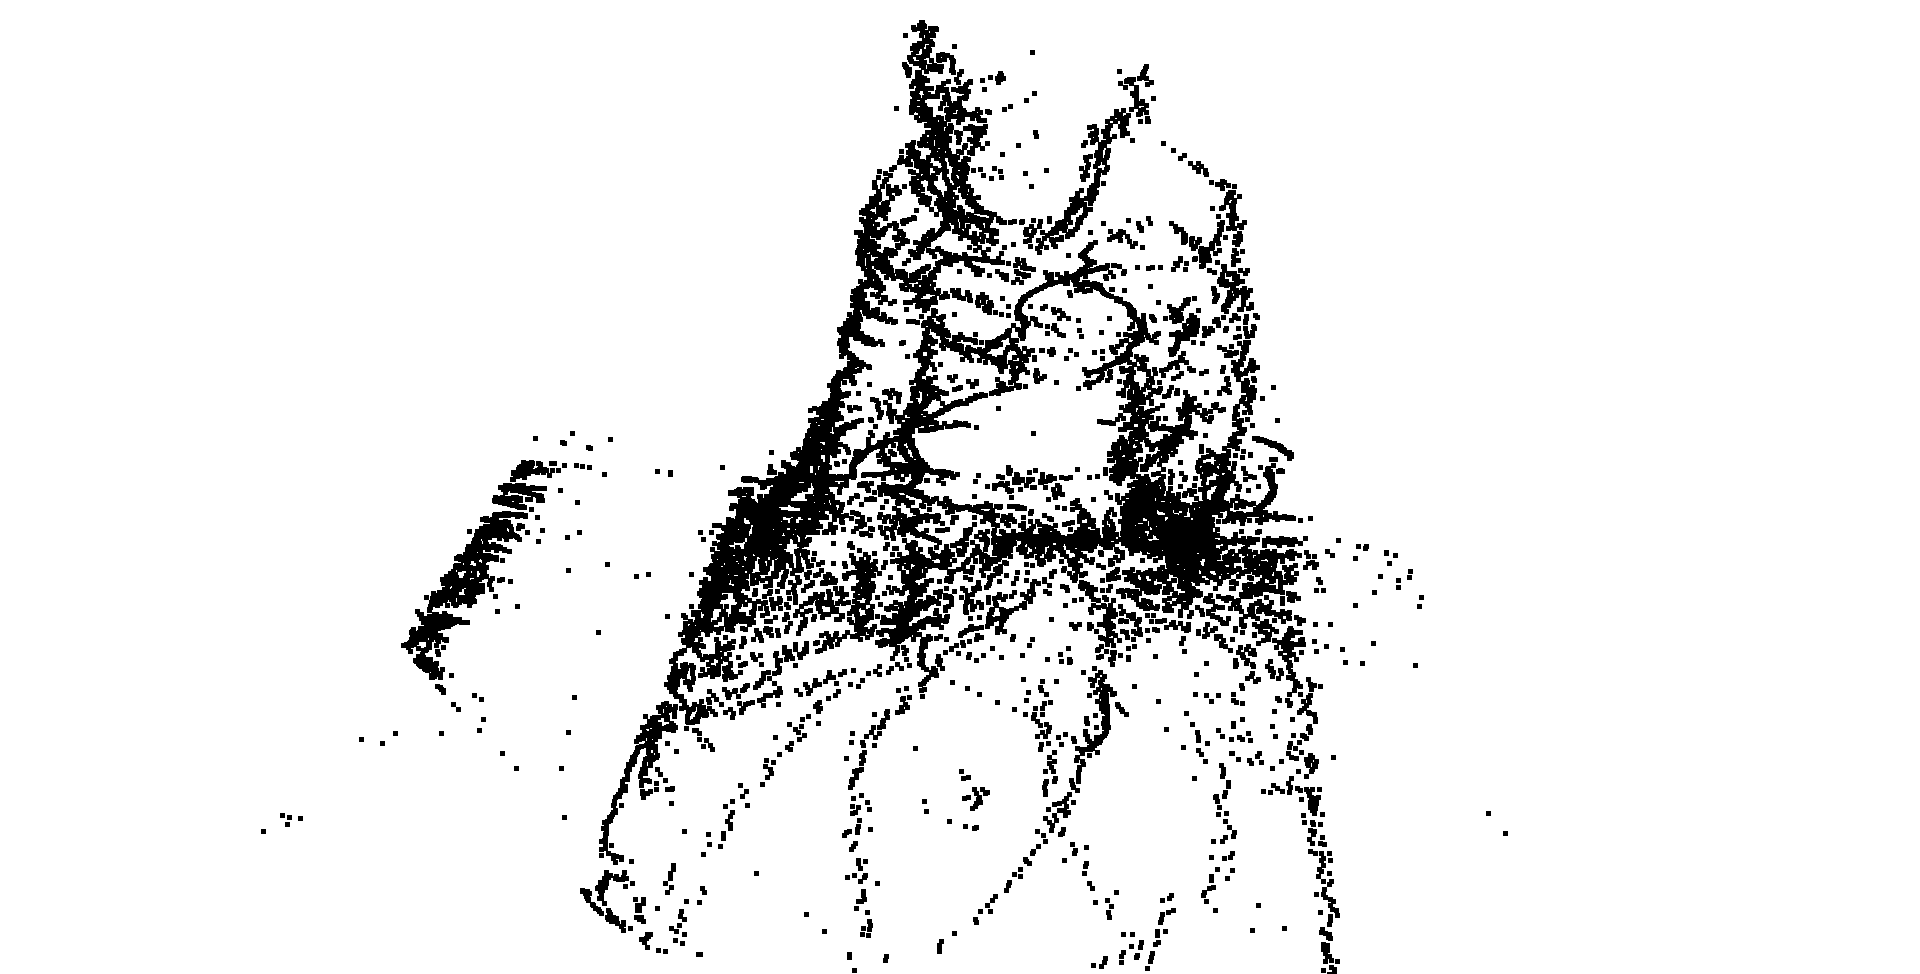
\includegraphics[width=.45\linewidth]{img/mouse.png}
    \label{pcmouse}
  }
  \subfloat[Pad operation]{
    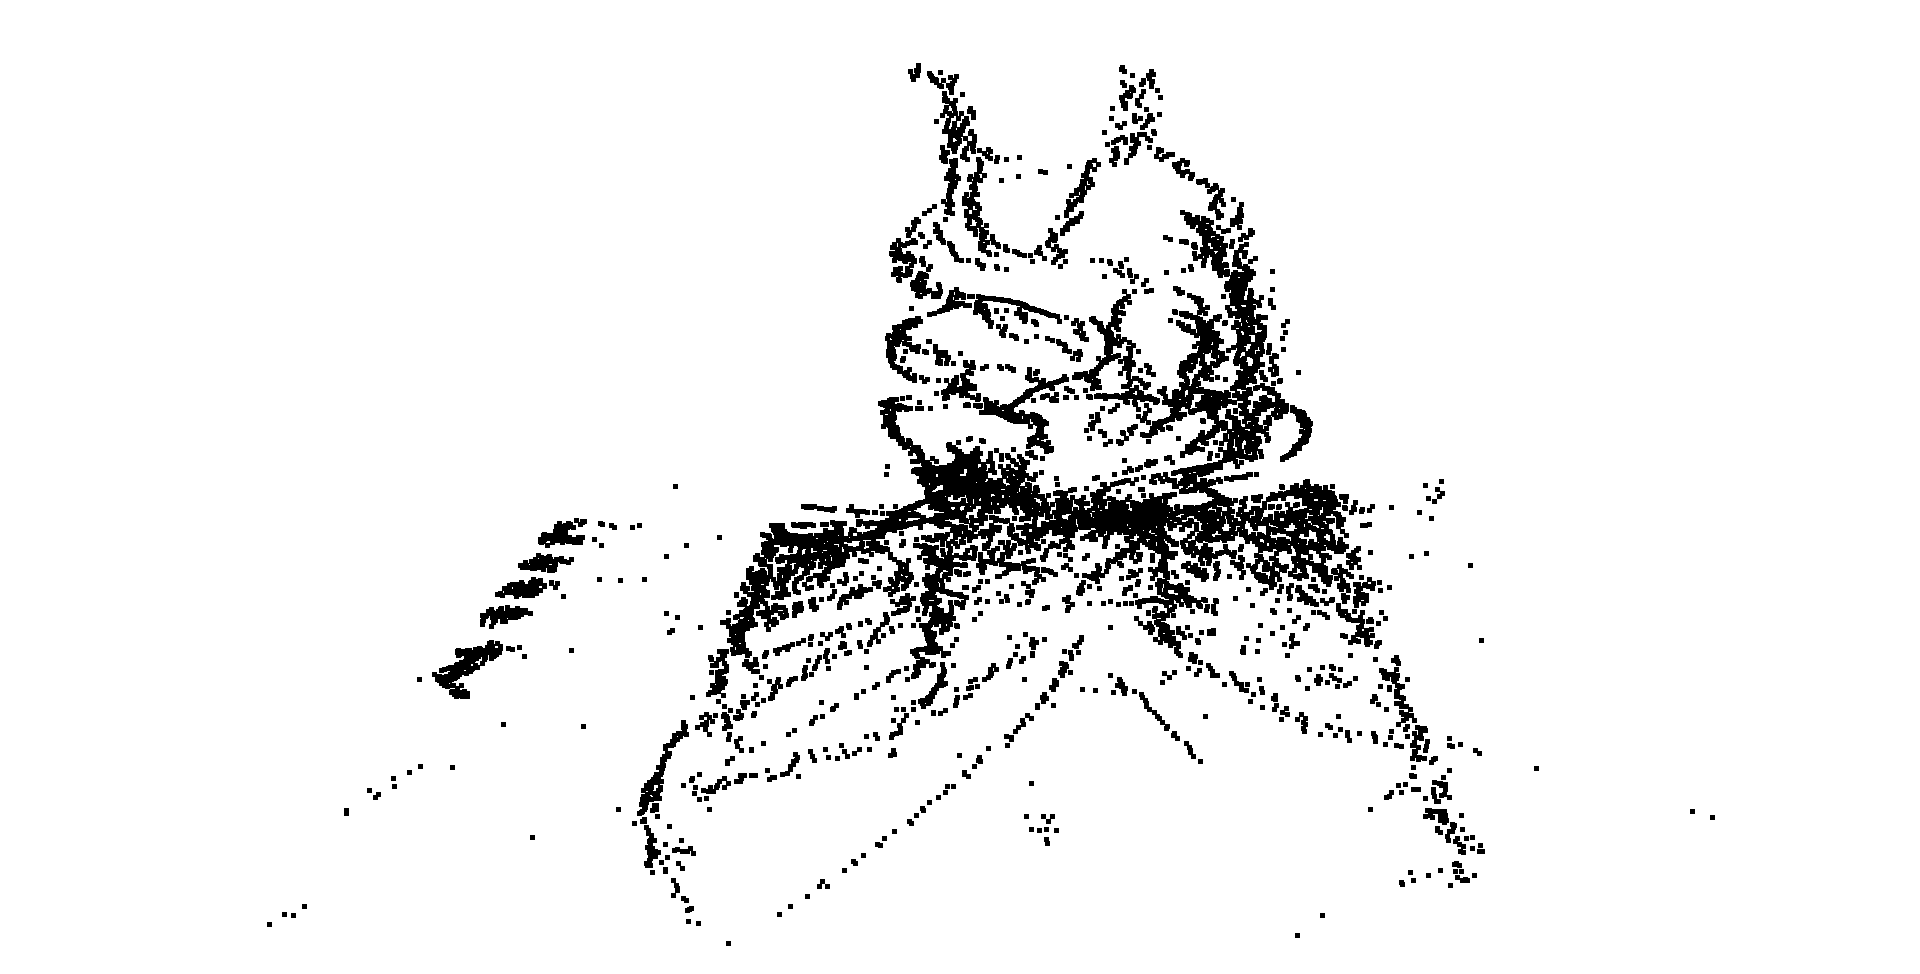
\includegraphics[width=.45\linewidth]{img/pat.png}
    \label{pcpad}
  }
  \\
  \subfloat[Sitting still]{
    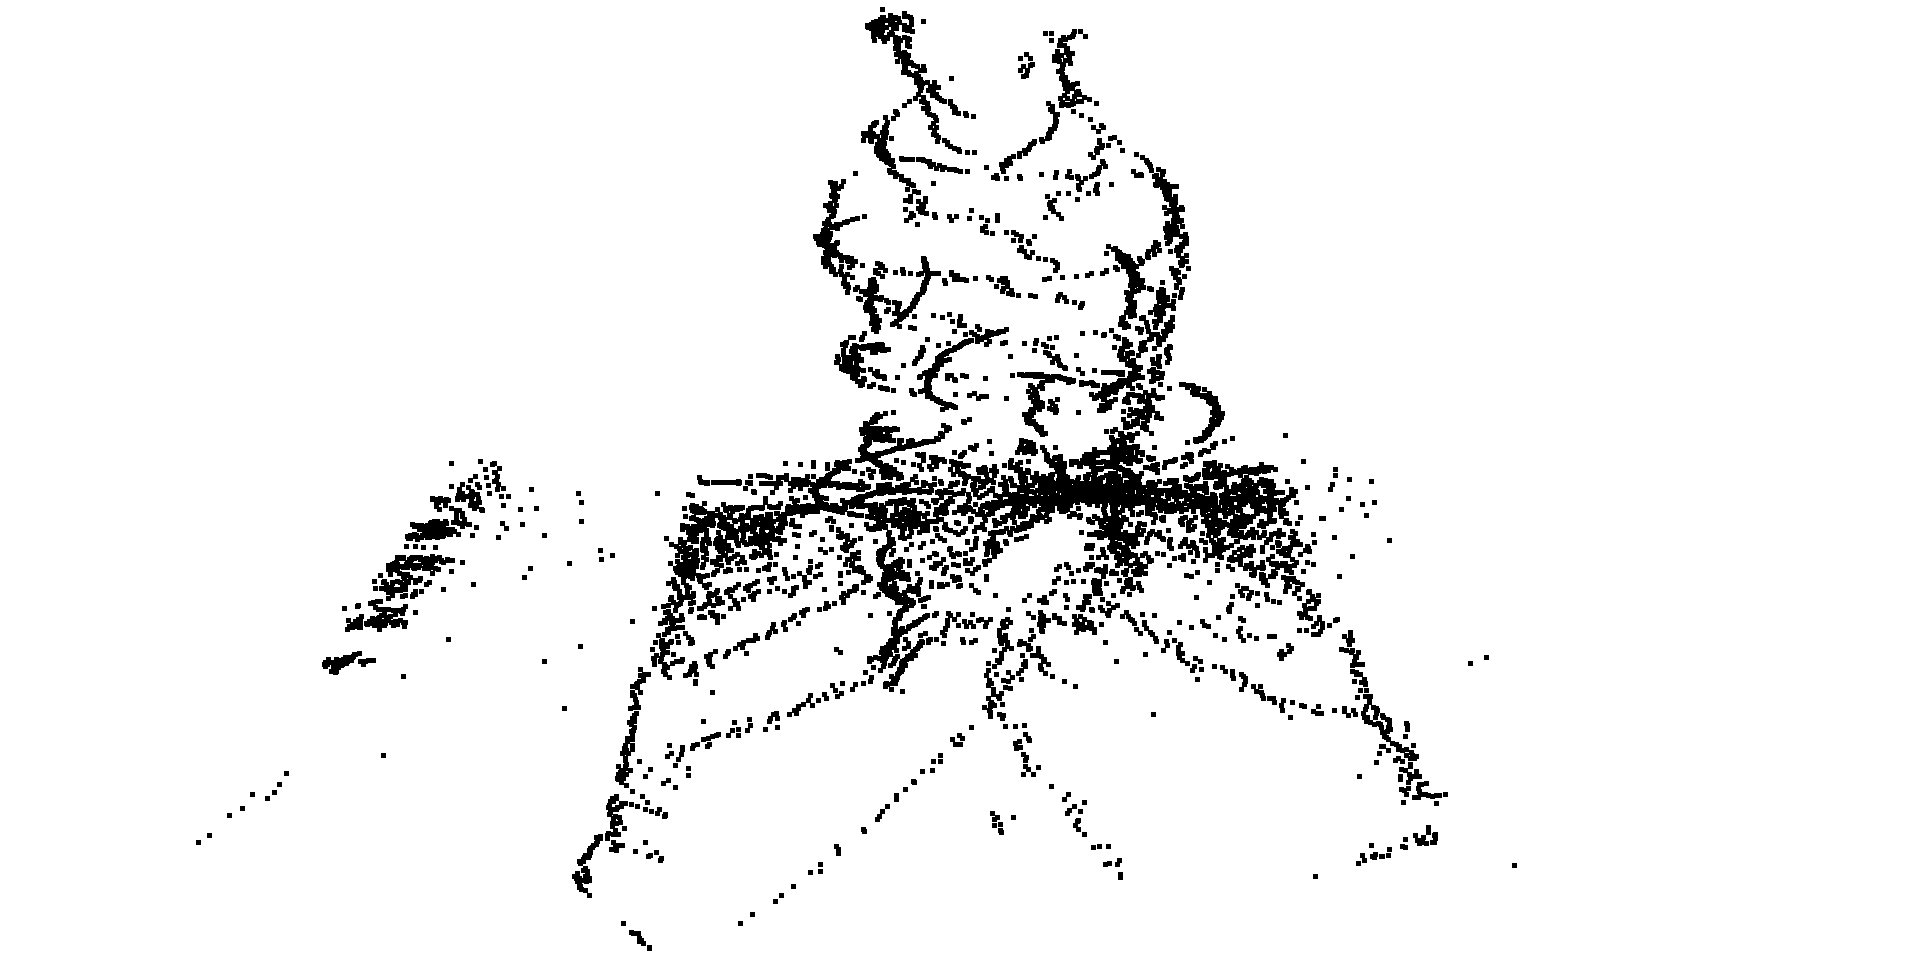
\includegraphics[width=.45\linewidth]{img/stay.png}
    \label{pcstay}
  }
  \subfloat[Typing]{
    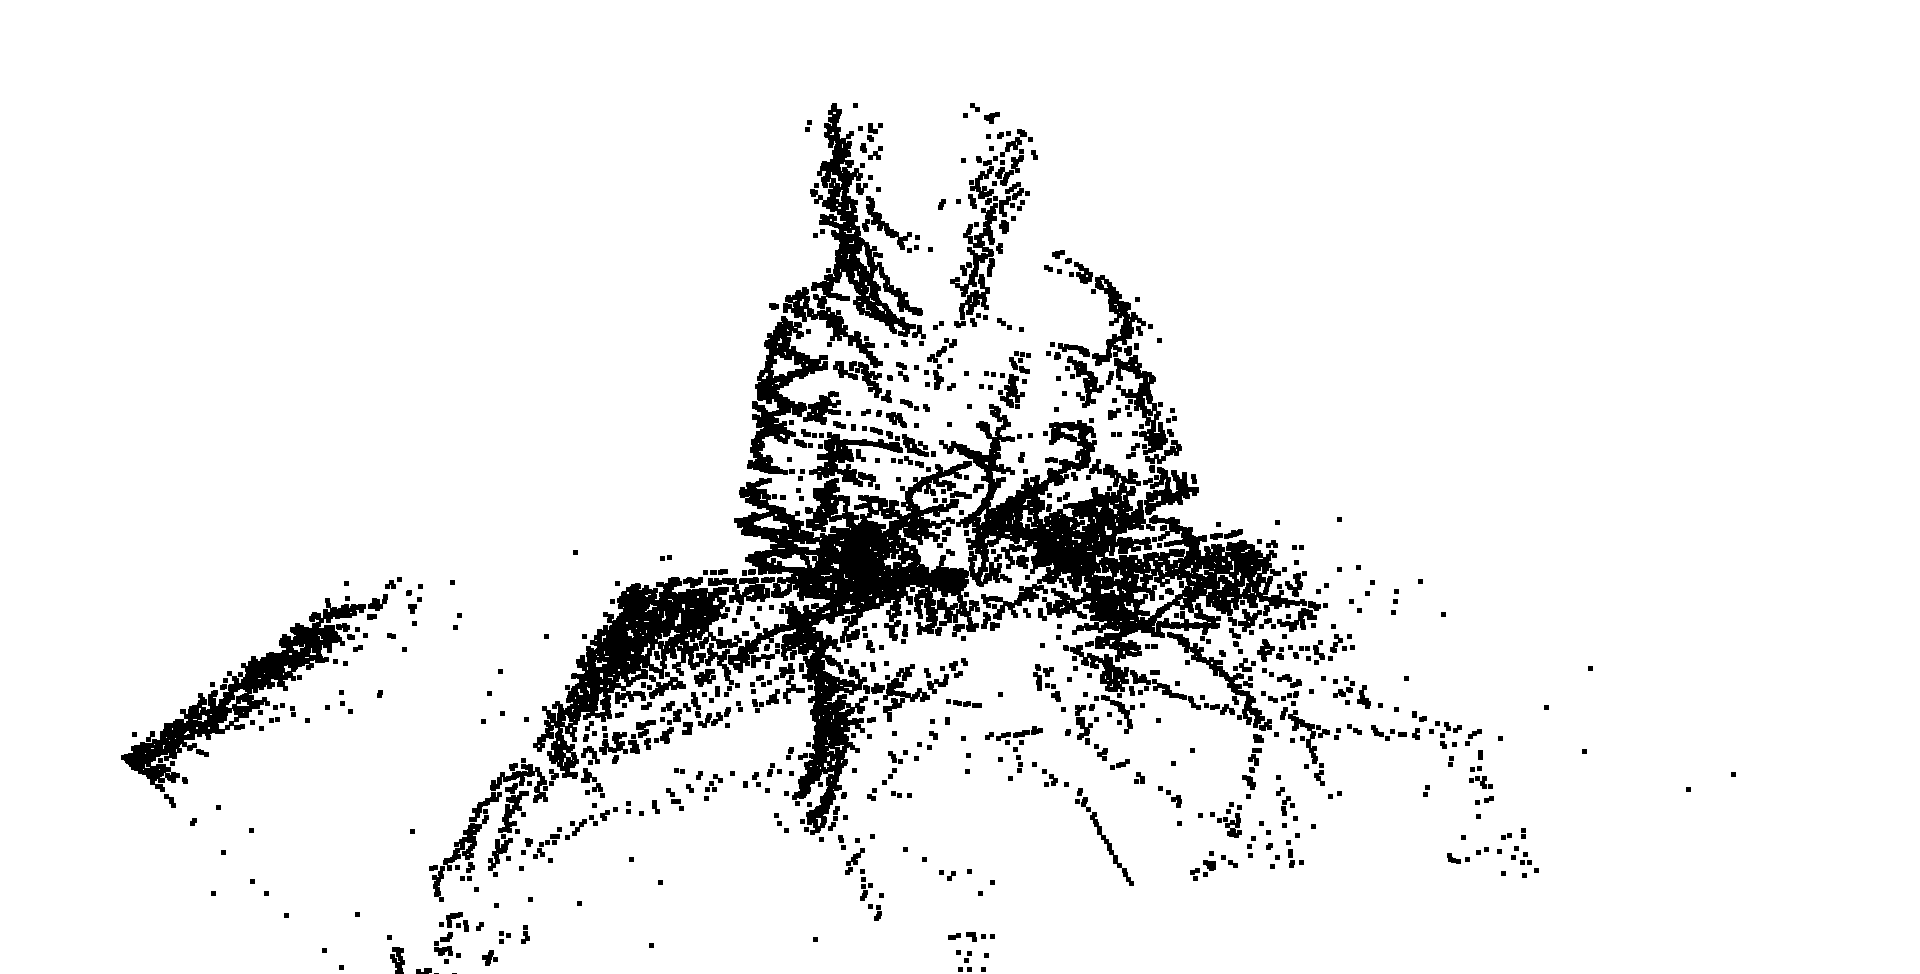
\includegraphics[width=.45\linewidth]{img/typing.png}
    \label{pctyp}
  }
  \caption{Visualization of data showing each label.}
  \label{labels}
\end{figure} 